\chapter{Space Combat}\label{sec:space-combat} % \href{sec:id136}

\begin{sidebox}{Original Material}

The \href{http://www.vsca.ca/Diaspora/Space%20combat%20demo.pdf}{original chapter about Space Combat}
is available from the Diaspora Website:
\begin{center}\verb#http://www.vsca.ca/Diaspora/Space%20combat%20demo.pdf#\end{center}
\end{sidebox}


Spacecraft are large, relatively fragile things pursuing their goals at high velocity in the dead of space. They are constrained by their available reaction mass, the mass  allocated for trade cargo, and their ability to dissipate heat. When they test each other to destruction using the assorted weapons of space combat --- beams, torpedoes, and electronic warfare --- they are chiefly pursuing goals of domination or escape. This system emphasizes these goals. The stories we want to tell include:

\begin{itemize}
\item an inferior ship escaping from the authorities
\item a hostile vessel capturing cargo
\item a threat so powerful the only real option is to surrender
\item a convoy of merchants and escorts safely defending itself from marauders
\end{itemize}

Space combat occurs on a simple map that emphasizes pursuit in order to provide a simple and fast system.

Combat occurs in phases. First is the detection phase which establishes the initial positions. Then the positioning, electronic warfare, beams, torpedoes, and damage control phases are repeated in order until everyone is happy, dead, or escaped. Order of action is controlled by social pressure: a player is designated caller for the fight and that person controls the transition from phase to phase (see sidebar on ``Social Initiative''). If a player wants to act in a particular phase, he announces his action. The advantage of going first goes to the one that speaks first. The advantage of going last goes to the person who speaks last. When the caller calls for a change of phase, it is possible that some players failed to act in time.

\section{The Crew}
\label{sec:the-crew}

Diaspora assumes that spacecraft have a fully functional crew aboard, who draw a salary and are able to man their stations competently.  There is no need to flesh them out unless there are role-playing reasons to do so, and player characters can work beside an undifferentiated crew happily.

Except as noted below, all combat crew positions on a ship are assumed to be staffed by someone with a \Skill\ level of 2.  PCs serving aboard such ships may use their individual \Skill\ levels, but if they choose not to (e.g. if they ride as passengers), there is always someone who can do the job.

A ship's \Trade\ value is not used in combat, and therefore there is no default broker aboard to assist with maintenance rolls.

The exception to this is a spacecraft that has the \stunt{Skeleton Crew} \Stunt, in which case all the jobs in combat must be taken by a known individual (either a player character or an NPC who has been developed) who is trained in the relevant \Skill. In particular, \skill{Communications} and \skill{Gunnery} stations, if they have a positive value, may not be operated by an untrained individual.

For each crew position, there is only ever one person doing a given job at a given time. One Navigator rolls in the detection phase, and only one Computer expert rolls to repair the \Data\ track.

A PC may occupy more than one position on the ship, but it becomes challenging during combat. Each \Skill\ associated with a combat phase normally requires a single crew member to staff it.

\rulebox[Staffing more than one post earns a -1 cu\-mu\-la\-tive penalty to 
effective Skill level]{Staffing more than one crew position during combat earns a -1
cumulative penalty to the effective Skill level.}
For example, a gunner may fire beams offensively and defensively without penalty, but would receive a penalty on the torpedo roll if he has fired beams.

\rulebox[Each crew member may act once per phase]{Each crew member may only act once per phase in combat.}
For example, a single gunner may not fire beams defensively and launch torpedoes in the same phase.


\section{Spacecraft}
\label{sec:spacecraft}

Spacecraft are the unit of scale in this mini-game, and not player characters. They have their own \Skills\ (\Vshift, \skill{Electronic Warfare}, \skill{Beams}, and \skill{Torpedoes}), \Stunts, \Aspects\ and stress tracks (\Frame, \Data\ and \Heat). The mini-game will involve rolling those \Skills to achieve results and marking damage against those stress tracks.

Spacecraft can mitigate stress hits with three \Consequences, just as characters do. You will find a list of ships at the end of the chapter, and later a method for creating your own.

Spacecraft not designated as \stunt{Civilian} can only be flown by characters with the \stunt{Military-grade Pilot} Stunt. Further, offensive use of the \skill{EW} ship Skill can only be done by characters with the \stunt{Military-grade EW} Stunt. Aspects listed are meant as suggestions: every ship has its own quirks and personality.


\section{The Map}\label{sec:social-combat-map}
% \vfil

Social combat takes place on a zone map much as it does with personal combat. Instead of representing some physical geography, the map represents the social space of the encounter. Because of the kinds of options available to characters involved in social combat, certain kinds of map shapes have certain kinds of effects on behaviour and can be used to represent specific issues.

In general, concentric circles imply intimacy. Zone shapes with many borders, and therefore many avenues of escape and access, better represent socially open places like chatting about the weather at a party. Intimate zones are often objectives, such as when you want to get someone to reveal valuable information, and so you want to maneuver them into intimate, trusting conversation.

% \newpage

To begin with, moving between zones has no additional cost --- there is no initial use of ``borders'' as there is in personal combat. Characters in the same zone can be said to be engaging each other socially: they are conversing about interesting, relevant things that they care about. Conversely, the further apart characters are on the map, the more social distance is in their conversation. Range has a deep impact on the effectiveness of characters' interactions and so one must usually close the range before one can do anything useful, such as move the conversation to a more intimate space.

% \newpage

Zones represent in the first instance a degree of intimacy in the social context. This will sometimes correspond to a spatial dimension too, but more often it represents something much more nebulous. For instance, a separate zone might correspond to a small balcony where a conversation might occur. It is often a good idea for the table to design the map of the social combat as a group.

Optionally, once the map is created, each player may choose to place one free-taggable \Aspect{} on a single zone, or a pass value of 2 on a single border, to reflect the personal contours of the social situation.

% badbox here
% \newpage

\subsection{Time}\label{sec:Time}

For each zone on the map, create one time box to represent available time to resolve. If you need to know exactly how long something took, the table should determine the maximum amount of time something is allowed (even the best party will disperse by morning). If a victory condition is achieved before the time boxes run out, the maximum time can be downgraded a number of shifts on the Time Track (Dealing With Time, Chapter 2) equal to the number of unchecked boxes. Often, table consensus will determine a very similar result in any case.

% \newpage

\subsection{The Actors}\label{sec:The Actors}

One of the biggest conceptual hurdles in adopting this system for resolving social interactions is recognizing that not every person in a scene needs to be represented on the map. Part of this is embodied within the zones themselves, as \Aspects{} on the zones can represent the other people involved.

This can in fact be made even more abstract, when you want to make a situation tactical that has become mired or unproductive in regular role-play. By making some of the actors on the map ideas instead of explicit people, you can conduct a scientific investigation or any other information-revealing multi-step endeavour. Make the opposition the Fact and, maybe, an Attractive Falsehood and you can do science. Add in people with conflicting goals (a young whipper-snapper who wants to be primary author on the publication of your discovery!) and the abstract can engage the concrete in both directions.

% \newpage

\subsection{Victory}\label{sec:Victory}

Victory conditions should relate to map position. Usually the objective will be to get a certain person or persons into a specific zone before the timer runs out. This can be more complex, however, to achieve different goals: if you want to model persuading a crowd, you could score participants by how many crowd members are in their target zone when the timer runs out. Feel free to push the system around and find other victory conditions.

\newpage

\subsection{Sample Maps}\label{sec:Sample Maps}

% \newpage

\subsubsection{Party}

A party has a lot of accessible conversation space --- everyone is there to chit-chat after all --- and probably at least one intimate space. It is well represented by a central shape with several attached shapes. Inside one attached space, add a couple of concentric circles for intimacy. An objective in the party might be to hook up with a powerful businessman and get him to brag about his company's secret operation on the dark side of the moon: you win if you can get him, yourself, and the science officer into the center of the intimate zone before the timer runs out.

The party map doesn't need to be complicated --- the simpler it is the faster things will go. The important thing is to make it take a few steps to get to the target zone and be complex enough to imply story with every move. The map above is about the minimum complexity you would want from a social combat map. It might be close to the maximum also!

% \newpage

\subsubsection{Seduction}

\begin{figure}
\centering\footnotesize
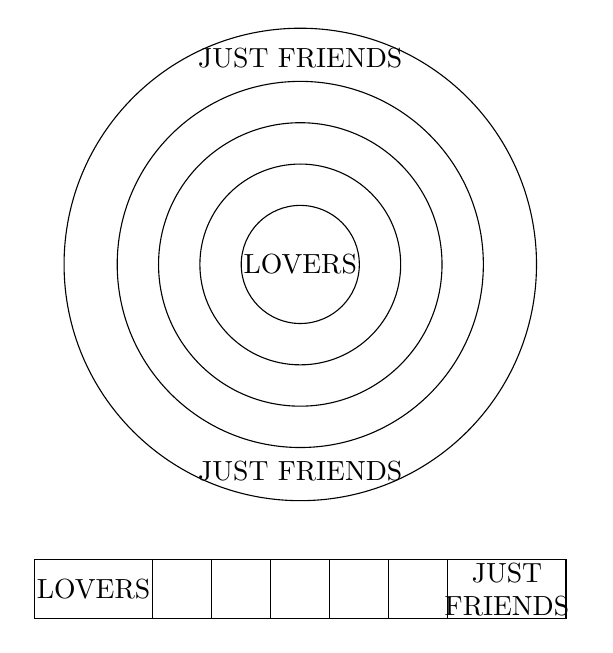
\begin{tikzpicture}[scale=0.75]
\begin{scope}
\draw circle (1) circle (1.7) circle (2.4) circle (3.1) circle (4.0)
  (0,0) node {LOVERS}
  (0,3.5) node {JUST FRIENDS}
  (0,-3.5) node {JUST FRIENDS};
\end{scope}
\begin{scope}[yshift=-5cm]
\draw
  (-2.5,0) rectangle +(-2,-1)
    +(-1,-0.5) node [anchor=center] {LOVERS}
  (2.5,0) rectangle +(2,-1)
    +(1,-0.5) node [text width=1.75cm,text centered] { JUST FRIENDS}
  \foreach \x in {-2.5,...,1.5} {
    (\x,0) rectangle ++(1,-1)
  }
;
\end{scope}
\end{tikzpicture}

\caption{Sample social combat map: Seduction}
\label{fig:social-combat-map-seduction}
\end{figure}

% \newpage


A seduction might be well modeled with a deep set of concentric circles --- say five or six --- with the objective of getting both characters in the bull's-eye (such as in \autoref{fig:social-combat-map-seduction}). Such an engagement could have multiple suitors and possibly require removing some or all from the map through Composure damage.

Suitors might be PCs or they might be NPCs or in some cases they might just be ``pawns'' --- if there is a concept you want to be relevant to the goal but that doesn't necessarily need to have free will in the fight, just give it a marker and no statistics. Players can move it around towards or away from goals (voters in an election or observers at a debate!) but it doesn't do anything on its own.

This could also be done with a simple linear track of, say, seven zones. Mark the first zone \LOVERS{} and the last zone \JUSTFRIENDS{}. Start the seducer on or near \LOVERS{} and the objective on or near \JUSTFRIENDS{}. Start other competitive suitors anywhere that seems fun or scary.

If the objective and anyone else are together on the \LOVERS{} zone, it has fallen for that suitor. If the objective and anyone else are together on the \JUSTFRIENDS{} zone, whoever has joined the objective there is removed from play.

% \newpage

\subsubsection{Debate}

\begin{figure}
\centering\footnotesize
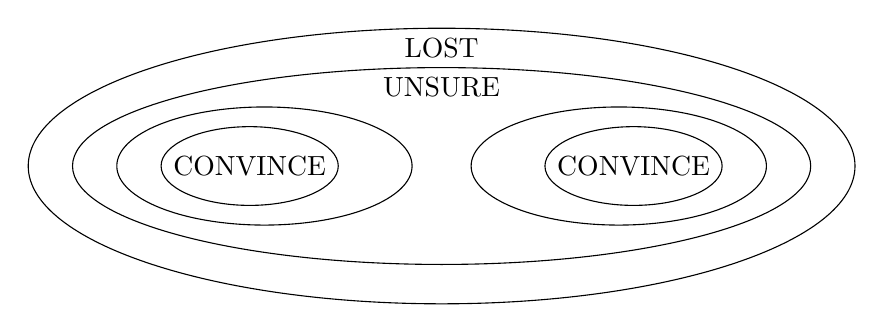
\begin{tikzpicture}[xscale=0.75,yscale=0.5]
\begin{scope}
\draw
  (-3,0) circle (2.5 and 1.5)
  (-3.25,0)   circle (1.5 and 1) node {CONVINCE}
  (0,0) ellipse (7 and 3.5) (0,3) node {LOST}
  (0,0) ellipse (6.25 and 2.5) (0,2) node {UNSURE}
  (3,0) circle (2.5 and 1.5)
  (3.25,0)   circle (1.5 and 1) node {CONVINCE}
%   (-3,0) node {CONVINCE}
%   (0,3.5) node {JUST FRIENDS}
%   (0,-3.5) node {JUST FRIENDS}
;
\end{scope}
% \begin{scope}[yshift=-5cm]
% \draw
%   (-2.5,0) rectangle +(-2,-1)
%     +(-1,-0.5) node [anchor=center] {LOVERS}
%   (2.5,0) rectangle +(2,-1)
%     +(1,-0.5) node [text width=1.75cm,text centered] { JUST FRIENDS}
%   \foreach \x in {-2.5,...,1.5} {
%     (\x,0) rectangle ++(1,-1)
%   }
% ;
% \end{scope}
\end{tikzpicture}

\caption{Sample social combat map: Debate}
\label{fig:social-combat-map-debate}
\end{figure}

% \newpage

A debate can be modeled with two sets of concentric circles representing opposing perspectives (see \autoref{fig:social-combat-map-debate}). The objective would be to move the opponent into your own central circle or moving the majority of audience members into your zone. Note that because of the steep drop-off in effectiveness at range, it will be necessary to move towards your opponent in order to engage him and pull him back to see your point (answering his specific arguments, showing sympathy and understanding).


% \section{Social Initiative}
\vfil\begin{sidebox}{Social Initiative}

\label{sec:Social Initiative}

The space combat mini-game operates using a form of social initiative. While often it is possible for the caller to start with one player who wants to act first and to proceed simply around the table, the stalemate-inducing anxieties of the uncertain commitment of resources over time can be fun to play with --- it creates the eerie feel of submarine combat, reducing the information available as decisions get made. For each of phases 1-4, the decision to act first resides with the player who states that they act first, with the caller determining priority if more than one person speaks at a time (or the table if the caller is controlling one of the affected ships).

% \rulebox{Resources, once com\-mit\-ted, can only be in\-creased.}

Going first entails a commitment of resources, and responses to the initial action can be proportionate, using the information of how much the first player has committed.
Resources, once committed, can only be increased.
They are never decreased.

As each phase ticks by, players may hold back attacking to wait until they see if they are being attacked and by how many, or they may strike hard and fast, filling their Heat track and hoping for a quick kill (or escape!).
\end{sidebox}

\section{The Sequence}\label{sec:The Sequence}

Space combat is played in turns, each of which might represent fifteen to thirty minutes of in-game time --- this too has been largely abstracted. Each turn consists of several phases, and each phase will offer a test --- an opportunity to cross-compel, a roll, and an opportunity to tag and/or invoke \Aspects.

\subsection{Detection}
\label{sec:Detection}

% \makeatletter
% \newsavebox{\hbbox}%
% \begin{lrbox}{\hbbox}
% \begin{minipage}[c]{3.8cm}
% \sideboxtitle{Phases}
% The phases are:
% \begin{enumerate}
% \item Detection
% \item Position
% \item Electronic warfare
% \item Beam
% \item Torpedo
% \item Damage control
% \end{enumerate}
% \end{minipage}
% \end{lrbox}
% \begin{wraptable}{r}[\sidebarwidth]{0cm}\end{wraptable}
% \makeatother

% ~

\begin{wraptable}{r}[\sidebarwidth]{5cm}
\centering
% \begin{halfbox}{r}{5cm}{Phases}
\newsavebox{\hbbox}%
\begin{lrbox}{\hbbox}
\begin{minipage}[c]{4.5cm}
\sideboxtitle{Phases of space combat}
% The phases are:
\begin{enumerate}
\item Detection
\item Position
\item Electronic warfare
\item Beam
\item Torpedo
\item Damage control
\end{enumerate}
\end{minipage}
\end{lrbox}
\colorbox{sbbackground}{\usebox{\hbbox}}
% \caption{#5}
% \label{#6}
% \end{halfbox}
\end{wraptable}

Before a fight can start, everyone needs to find each other. Position is plotted on a linear scale from -4 to +4 on the map. As always, before any dice are rolled, the caller will ask for compels, at which time players can compel each other to fail to act. Failure to act in this case is represented by an automatic result of -4 (dice are not rolled and \Skills\ are not considered: your final result for your \Navigation\ check is -4).

A \Navigation\ check is rolled by each ship's navigation officer, and all rolls are ranked. Ties are resolved by raw \Navigation\ \Skill. The highest ranked Navigator will place two of the ships to be played on the map anywhere except the two most distant lines (-4 and 4). The next highest rank then places a single ship and this continues until all ships are placed. The lowest ranking Navigator places nothing. The ship which wins the detection round may also decide if there will be a positioning roll in the first turn (only). Once all the ships are placed, the winning ship in this phase decides whether to proceed to phase 1 or directly to phase 2. This allows a ship to attempt escape without engaging in combat immediately on being detected --- going to phase 1 --- or it allows it to use the tactical position from the detection phase for an optimized initial combat round --- going to phase 2.

In the event of a tie between two ships (as might happen when two standard T2 merchant ships meet, with default navigators), if neither ship is willing or able to invest fate points to gain victory, ships are placed randomly, based on a roll of the fate dice (it is only in this circumstance that a ship may begin at the 4 or -4 band).

\subsection{Position}\label{sec:Position} % \href{sec:id143}

As always, before any dice are rolled, the caller will ask for compels, at which time players can compel each other to fail to act. Failure to act in this case is represented by an automatic result of -4 (dice are not rolled and Skills are not considered: your final result for your positioning check is -4).

Spacecraft positions are plotted on a simple linear scale from -4 to +4. Ships begin as they were placed in the detection phase. At the beginning of each round of combat, pilots jockey for position. All pilots roll their ship's V-shift rating limited by their effective Pilot Skill (i.e. if one character is serving both as Navigator and Pilot, then the Pilot's effective Pilot Skill is reduced by one). Note also that this is not simply a modifier to the roll: since V-shift is limited by effective Pilot Skill, this penalty might affect performance for the first turn as well.

In addition, ships may apply burn: by running their drives over rating, they can exchange Heat for an advantage in maneuver, improving the V-shift roll. Any ship may declare that it is applying burn, state the value and add that value to their roll (not to the V-shift rating). They immediately take a hit to their Heat stress track equal to the value of their burn, marking that box and all unmarked boxes below it. If the highest box to be marked is already marked, mark the next higher open box. Before marking the damage to the Heat stress track, the pilot may reduce the detrimental effects through Consequences exactly as mitigating combat damage. The caller may allow negotiation of burn declarations at his preference, though generally a declared burn rating by a ship's player must stand.

Ships may choose not to use their drives in order to bleed heat. Each turn that the V-Shift is not engaged allows the highest filled box in the Heat track to be cleared immediately. This decision results in an automatic -4 final result for the positioning check, which might still be modified by Aspects, but no dice are rolled and no Skill is used. No burn declarations can be made once the caller declares the bidding closed and asks for dice on the table.

Only the highest roller may alter any ship's positions:
\begin{itemize}
\item He may move himself the difference between his roll and the lowest roll, or
\item He may move any ship with a lower roll up to the level of the
difference between them.
\end{itemize}

He may not, however, move any vessel more map bands than his own vessel's V-shift rating. Remember, moving a ship between the 3 and 4 bar (or the -3 and -4) costs 2 shifts, and moving a ship from the last bar off the map costs 3 shifts.

If the winning positioning roll is tied, the next highest roll is the winner. This presents some interesting tactical choices for fate point expenditure: sometimes it's advantageous to forfeit your awesome roll so that your ally, who rolled lower, can make use of his better V-shift, for example. You might then use an Aspect to force a tie so that you lose control.

If a ship exceeds the band at -4 or 4, they leave combat, whether forced off by others or maneuvered off by their own pilots. In this fashion a really excellent pilot in a hot ship can cut down the odds by positioning enemy vessels off the map until he faces only one opponent. Similarly, more than two ships chasing a single ship can usually keep the lone opponent on the map through positioning.

\subsection{Electronic Warfare}\label{sec:Electronic Warfare}
\vfil
As always, before any dice are rolled, the caller will ask for compels, at which time players can compel each other to fail to act. Failure to act in this case is represented by the ship being unable to declare a target.

Before any destructive weapons are used, each ship may conduct electronic warfare, pitting its communications officer against the enemy. If a communications officer has \stunt{Military-grade Communications}, she may pick a target and roll the ship's \skill{Electronic Warfare} (EW) rating, amplified by her effective \skill{Communications} Skill (if the communications officer has acted in any of the previous phases, there is a cumulative -1 penalty for each phase she has acted). The defender also makes a roll, of his ship's \skill{EW} rating, amplified by the communications officer's effective \skill{Communications} Skill. The rating may be zero, in which case there is there is no crewman staffing the position unless this is done by one of the PCs. Ships may have a Stunt (\stunt{Firewall}) that automatically provides a defense value of 2, and which may not be modified. Subtract the defender's modified roll from the attacker's.

As with any roll, these results can now be modified by tagging or invoking \Aspects\ and paying a fate point to get +2 or re-roll.

Positive values are treated as shifts against the defender, and
%
negative values are treated as shifts against the attacker.
%
Whoever has shifts against him will take a \Data\ stress track hit to the ship. Before damage is calculated, the player may apply \Consequences\ to reduce the number of shifts: a mild Consequence reduces the shifts by one, a moderate Consequence reduces the shifts by two, and a severe Consequence reduces the shifts by four. Recall that no entity can have more than three Consequences of any kind and never more than one of each type.

% \newpage

Once the final number of shifts are determined, the corresponding box on the \Data\ stress track is marked and all open boxes below it are also marked. If the highest box to be marked has already been marked, mark the next highest open box.

Note that only one roll is made for each ship, so in some cases with more than two ships in play, a single roll may defend against multiple attacking rolls as well as conceivably acting as the attacking roll on a declared target. Note also that a good defense against hacking can inflict damage on the attacking \Data\ stress track, even if the defending communications officer does not have Military-grade \skill{Communications}.

The Electronic Warfare (EW) defense roll is persistent through this phase, but the total may be added to over the course of the phase through the spending of fate points. An outnumbered ship may still mount a reasonable defense.

% \newpage

\subsection{Beam Weapons}\label{sec:Beam Weapons} % \href{sec:id145}

Beam weapons subsume all relatively short range unguided weaponry, so they may be described as lasers of various wavelengths, artillery, rockets, railguns, electromagnetically propelled storms of small projectiles, particle beams, or anything else that suits the setting developed at the table. Beams are used both offensively, to directly damage targets at shorter ranges, and defensively, to defend against torpedoes (see Torpedo phase for details).

As always, before any dice are rolled, the caller will ask for compels, at which time players can compel each other to fail to act. Failure to act in this case is represented by a failure to declare a target in whatever phase the player ship was compelled.

A ship with a Beam Skill can attack at any value from 1 up to the full Beam rating. When Beams are fired offensively the attacker must declare what Beam rating he will apply. Note the Beam value used, as it will be relevant in the Torpedo phase.

All combat rolls are made at the Beam rating amplified by the gunner's Gunnery Skill (that is, the Beam rating is used and increased by one if the Gunnery Skill is higher). If the gunnery officer has acted in any of the previous phases, there is a cumulative -1 penalty to the effective Skill level for each phase he has acted. 

Beams firing at three or more bands range subtract 2 from the roll. Attacks are resolved as they are declared, again leveraging social pressure to determine who goes first: the caller closes the call for targets by announcing a final call, and counting slowly to three (if necessary --- if your caller is fair and fun, he'll leave plenty of time), after which no further targets can be announced.

There is no skill to defend against Beams. A roll with no modification is made to oppose all incoming Beam attacks. Ship's may have a Stunt (Vector Randomizer) that changes the base from 0 to 2.
Defensive rolls are made once for each defensive system but stay on the table --- that defensive roll you made against Beams stands throughout the Beam Weapons phase, complete with any modifications from invoking Aspects, using spin, etc. Defensive rolls are persistent through the phase, so it can be handy to note them on the ship card or use a coloured 12- or 20-sided die set to the result. Sometimes we write them on the map. Offensive Beam rolls are distinct from defensive Beam rolls (from the Torpedo phase) and should be recorded separately.

% \newpage

Subtract the defender's final sum from the attacker's to find the number of shifts, and thus the amount of stress on the defender's \Frame\ track. The defender may reduce these by applying one or more Consequences:
\begin{itemize}
\item reduce the shifts by one by applying a mild Consequence
\item reduce the shifts by two by applying a moderate Consequence
\item reduce the shifts by four by applying a severe Consequence.
\end{itemize}

Recall that no entity may have more than three Consequences and never more than one of each kind.

% \newpage

\subsection{Torpedoes}\label{sec:Torpedoes} % \href{sec:id146}

As always, before any dice are rolled, the caller will ask for compels, at which time players can compel each other to fail to act. Failure to act in this case is represented by a failure to declare a target in whatever phase the player ship was compelled.

Torpedoes attack at the spacecraft's Torpedo Skill rating, amplified by the gunner's effective Gunnery Skill (that is, the Torpedo rating is used and increased by one if the effective Gunnery rating is higher). If the gunnery officer has acted in any of the previous phases (including the Beam phase), there is a cumulative -1 penalty for each previously active phase.

Torpedoes firing at one or zero bands range subtract 2 from the roll. Attacks are resolved as they are declared, again leveraging social pressure to build an initiative order as in the Beam phase. The caller closes the call for targets by announcing a final call, and counting slowly to three, after which no further targets can be announced.

A Beam roll is made to oppose all incoming Torpedoes. To do this, the beam position must be staffed. If Beams were fired in the Beam Weapons phase, then the roll may be made as usual, amplified by gunner's effective Gunnery Skill. If Beams were not fired, then there must be a trained crew member available to man the beams in this phase: normal penalties and bonuses apply, but since each crew member may only act once per phase, a ship with a single gunner (as might happen with a skeleton crew) may have to choose between offensive Torpedo fire and defensive Beam fire. Beams so used may also have been fired offensively, and defensive fire may cause damage to the Heat stress track. Ships with no Beam rating or those unwilling to fire Beams defensively, roll with a base of 0 unless they have a Stunt (Point Defense) that changes the base from 0 to 2.

Defensive rolls are made once for each defensive system but stay on the table --- that  defensive roll you made with the Beams stands throughout the Torpedo Phase, complete with any modifications from Aspect invocation, spin, or other sources. As these rolls are persistent through the phase, it can be handy to note them on the ship card or use a coloured 12- or 20-sided die set to the result. Sometimes we write them on the map. Though persistent, defensive rolls are distinct from offensive rolls and should be recorded separately.

% \newpage

When Beams are fired defensively the attacker must declare what Beam rating he will apply. He may apply any value from 0 to the full Beam rating. Note the Beam value used. If the sum of the offensive Beam used in the Beam phase plus the defensive Beam used in the Torpedo phase is greater than the total Beam rating, then the ship takes a hit on the Heat stress track equal to the difference and marks all boxes below as well.

Subtract the final defender's sum from the attacker's to find the number of shifts, and thus the amount of stress on the defender's \Frame\ track. The defender may reduce these by applying one or more Consequences:
\begin{itemize}
\item reduce the shifts by one by applying a mild Consequence
\item reduce the shifts by two by applying a moderate Consequence
\item reduce the shifts by four by applying a severe Consequence.
\end{itemize}

Recall that no entity may have more than three Consequences, nor more than one of each kind.

% \newpage

\subsection{Damage Control}
\label{sec:Damage Control}

Damage control checks may now be made on Frame stress tracks (using one crew member's effective \skill{Engineering} Skill) or Data stress tracks (using one crew member's effective \skill{Computer} Skill). Since each crew may only staff one position per phase, the same individual may not be responsible for both rolls. If the engineer or computer officer has acted in any of the previous phases, there is a cumulative -1 penalty for each previously active phase. The target number for success is the highest box marked on the relevant track. The number of successes indicate the track box that can be erased. Erase it and all unmarked boxes below it.

The Heat stress track cannot be repaired during combat, except by shutting off engines, as described in the positioning phase.


\section{Damage}\label{sec:social-combat-damage}

Stress box hits are not real damage, but they can lead to Consequences. All stress box hits are removed after a few days of relaxing stress-free downtime. As with personal combat, the table should rule when enough time has passed or whether the downtime was sufficiently relaxing. Generally speaking it should be trivial.

\subsection{Recovering Consequences}\label{sec:social-combat-recovering-consequences}

A mild Consequence can be self-medicated with a bottle and some time alone once the scene is over. No roll is required and it is cleared as soon as the social combat scene is over.

A moderate Consequence remains until the end of the session in which it was incurred.

A severe Consequence must be carried through one complete session in which the associated stress track is never marked. If it is incurred during session one, it is gone no sooner than the end of session two, and if the associated stress track takes hit in a fight during that session, you'll need to hold the Consequence through yet another one.


\section{Special Maneuvers}
\label{sec:special-maneuvers}

\subsection{Formation Flying}
\label{sec:formation-flying}

Formation flying is a means of keeping two ships in the same range band at all times. Ships in formation may not be separated by the positioning rolls of another ship. This allows a merchant to fly with an escort, for example, or a fleet of fighters to maintain a common range for their attacks.

Ships may begin combat in formation. During set-up in the detection phase, any two ships (or more) in the same band may (but need not) be in formation, if the players controlling the ships so choose. Models are pressed next to each other to represent this.

Ships may enter formation with one another during the positioning phase. In the turn in which any ship is moved to band 0, and there is at least one other ship at band 0, the ship entering the band may enter formation with another ship.

Each pilot makes a roll, but the formation moves based on the lowest roll. If repositioned by another ship, the formation is moved as a unit. Ships in formation may only move as fast as the V-shift of the slowest ship allows.

A ship may leave formation at any time during the positioning phase. Formation flying allows all ships autonomy, but is more challenging to maintain than tethering in combat situations.

\subsection{Tethering}
\label{sec:tethering}

Tethering offers increased performance for ships in formation, at the expense of some autonomy for vessels. Tethering need not be physical, and any viable picture may be used to describe it: slaving the computer, perhaps; tethering could also be useful for slipping (``Convoy''). Two (or more) ships in formation may be said to be tethered, if one of the two following conditions are met: either both ships agree to be tethered and one agrees to lead, or one ship wishes to tether and lead and the other has been \TakenOut\ with a compatible narrated result.

There is always a primary ship when ships are tethered; one leads the other (or others). Multiple ships may be said to be tethered together, but only one can be leading. Only fate points from the lead ship can be spent while ships are tethered. As with formation flying, models are pressed together, but tethered ships gain the temporary Aspect \aspect{Tethered}. Tethered ships may not fire on other ships within their formation. They may be disengaged at any point, but only at the discretion of the leader. In the positioning phase, only the leader makes a piloting roll. Tethered ships may only move as fast as the \Vshift\ of the slowest ship, and may not initiate a burn.

\subsection{Boarding}
\label{sec:boarding}

In any turn, individuals from a lead ship may board any ship to which it is tethered. At this point, the game would normally revert to the individual tactical game: characters fight boarders! See Personal Combat (\autoref{sec:personal-combat}).

However, boarding can be addressed within the space combat game with an opposed roll, where any positive result for the boarders indicates the boarding action to be successful by the end of the following turn. Relevant \Aspects\ include \aspect{Boarding crew}, \aspect{Bunch of thugs}, \aspect{Tight security}, or \aspect{Elite marines}, but not \aspect{Tethered}. Ties favour the defending ship, however, and any ship that withstands a boarding party for three turns has repelled the boarders, and is no longer tethered. If it was tethered as a result of being \TakenOut, it remains \TakenOut, but requires new narration, this time provided by the defender since he succeeded in repelling boarders. These rules could also become applicable if the players stumble onto a boarding situation, or are asked to escort a target ship that is then attacked by pirates: the pirates board the target, while the characters in their ship maneuver about.

\subsection{Coupling}
\label{sec:coupling}

All ships have a nose coupling mechanism which may be attached to the base of the mast of any one other ship and can be used to tow (or, actually, push) the other ship. The coupled ship must be \TakenOut\ or tethered, and need not have a working drive.

Two coupled ships move at the lead ship's \Vshift\ rating -2. The lead ship gains the temporary Aspect \aspect{Slow to respond}, and the coupled ship's counter is removed from the map: the coupled ship may not fire weapons or take any other actions in the space combat game until it is decoupled. Ships couple or decouple during the positioning phase as an action. If ships decouple, the lead ship loses its temporary Aspect and regains full use of its \Vshift, and a counter is placed on the current range band to represent the decoupled ship. Derelicts are not placed on the map.


\section[Wargaming]{Wargaming}
\label{sec:personal-combat-wargaming}

Sometimes it's fun just to make one-off characters and have them shoot at each other. To play independently as a tactical war game, you need three things: a map, a story, and characters.

\subsection{The Map}
\label{sec:personal-combat-wargaming-map}

Someone is chosen as caller. Either the caller or the table draws a map. Is it a shoot out in an airport? A race to secure a bunker at the top of a hill? A boarding action in a submarine or a spaceship? Whatever the case, you need a map to play on.

You can start with a blank piece of paper, and take turns drawing features, until it looks good enough. Feel free to write words on the map too – these can become Aspects and help clarify what's what.

Once that is done, divide the map into zones. You don't want too many, but enough to allow opportunities for getting outside of range, and to allow movement. When drawing zones, it is often helpful to go from corner to corner: that means it is always clear when a character enters an area (from a door, or otherwise along a side) what zone he is in.

\subsection{The Story}
\label{sec:personal-combat-wargaming-story}

The process of drawing a map has already begun to determine what the story is: is this a fight to the death? Are there teams? Is most of the table maneuvering against a small cadre controlled by the caller (or by someone else)? Is there a difference in tech level between two sides? Whatever the case, articulating the story that is being told might mean that you go back and change the map slightly, add an Aspect to a zone or two, or whatever.

Most important is that the story articulates victory conditions, which need not be the same for all players. Is this a fight to the death? An attempt to capture someone alive? Someone working to escape detection and get out of a building, or sabotage a spacecraft's drives? Whatever the case, the victory condition might be defined in terms of time: get off the ship in eight turns; spend two turns alone in the engine room setting explosives.

\subsection{Characters in Wargaming}
\label{sec:characters-in-wargaming}

\iflandscape
{\begin{wraptable}[14]{r}[0.9\sidebarwidth]{5cm}}
{\begin{wraptable}[14]{r}[0.9\sidebarwidth]{5.5cm}}
% \begin{table}[ht]
\centering
\begin{tabular}{ll}\toprule
Skill & type \\
\midrule
Agility		\\
Alertness	\\
Brawling	& combat \\
Close Combat	& combat \\
Energy Weapons	& combat \\
EVA		\\
MicroG		\\
Resolve		& track \\
Slug Throwers	& combat \\
Stamina		& track \\
Stealth		\\
Tactics		\\
\bottomrule
\end{tabular}
\caption{Useful skills for personal combat wargaming}
\label{tab:personal-wargaming-skills}
% \end{table}
\end{wraptable}


Once the map and the story are determined, everyone should spend five minutes (no more) making one or two characters to push around the map.

\subsubsection{Skills}

Given the limited focus of this tactical game, 3-cap characters should be sufficient: pick one Skill at level 3, two at level 2, and three at level 1. Everything else is considered untrained. While any Skill might be taken, \autoref{tab:personal-wargaming-skills} presents Skills particularly relevant to this mini-game.

\subsubsection{Stress Tracks}

Characters should only concern themselves with the \Health{} and \Composure{} stress tracks. Each is three boxes long. If the character has \skill{Resolve} at level 1 or 2, the \Composure{} track has four boxes; if he has \skill{Resolve} 3, the \Composure{} track has five boxes. If the character has \skill{Stamina} at level 1 or 2, the \Health{} track has four boxes; if he has \skill{Stamina} 3, the \Health{} track has five boxes.

\subsubsection{Stunts}

Every character selects a Stunt. Making something Military-grade or altering how a stress track works are both obvious choices. (For some stories, it may be desirable to allow two Stunts per character; that's fine, as long as it's the same across the board).

\subsubsection{Aspects}

Each character should have three Aspects, revealed to all at the table. Each character also begins with three fate points.

Making a note card for each character, placed in front of the player with all the relevant information and a small pile of fate points stacked on top keeps all the information clear at all times. This is obviously scaled back from the RPG, and introduces a slightly different calculus for what constitutes a success. With reduced characters, teamwork, particularly in laying down maneuvers to be free-tagged, is rewarded.

